% Source: tex/chapters/ch05/00_chapter_opening.tex
\section{第05章 ソフトウェアテスト}
\begin{pointbox}{この資料の読み方}
専門用語は原則として日本語で示し、必要に応じて英語を括弧内に併記する。英語名は、元資料、試験範囲、ツール名を確認するときの手がかりとして残す。初学者が前提知識なしに読めるように、各節では「何を確認する活動か」「なぜその考え方が必要か」「実務では何に注意するか」を重視する。文体は、だである調に統一する。
\end{pointbox}

% Source: tex/chapters/ch05/01_全体概要：この章で学ぶこと.tex
\subsection*{全体概要：この章で学ぶこと}
\addcontentsline{toc}{subsection}{全体概要：この章で学ぶこと}
この章は、ソフトウェアテストを「実行による確認」として扱う。テストは、テスト対象システムを動かし、観測された結果と期待される結果を比べる活動である。ただし、現実のソフトウェアでは、すべての入力、すべての状態、すべての環境を試すことはできない。したがって、テストは常に、限られた資源でどのテストケースを選ぶかという判断を伴う。

\begin{pointbox}{到達目標}
この章を読み終えると、次のことができるようになる。
\begin{itemize}[leftmargin=2em]
  \item 欠陥、障害、テストケース、テストスイート、テストオラクルを区別できる。
  \item 単体テスト、結合テスト、システムテスト、受入テストの違いを説明できる。
  \item 仕様ベース、構造ベース、経験ベース、欠陥ベース、利用ベースのテスト技法を比較できる。
  \item カバレッジ、欠陥密度、信頼性成長モデル、ミューテーションスコアなどの測度の役割を説明できる。
  \item テスト計画、設計、環境構築、実行、インシデント報告、完了判断の流れを説明できる。
  \item 従来型開発、アジャイル、DevOps、TDD、クラウド、AI、ブロックチェーンなどでテストがどう変わるかを説明できる。
\end{itemize}
\end{pointbox}

初学者は、まず「テストは何を証明でき、何を証明できないか」を押さえるとよい。次に、テストのレベル、目的、技法を分けて理解する。最後に、測定、プロセス、ツールの話に進むと、個別技法が実務の中でどう使われるかを理解しやすい。

\begin{figure}[htbp]
\centering
\IfFileExists{assets/fig-ch05-01.png}{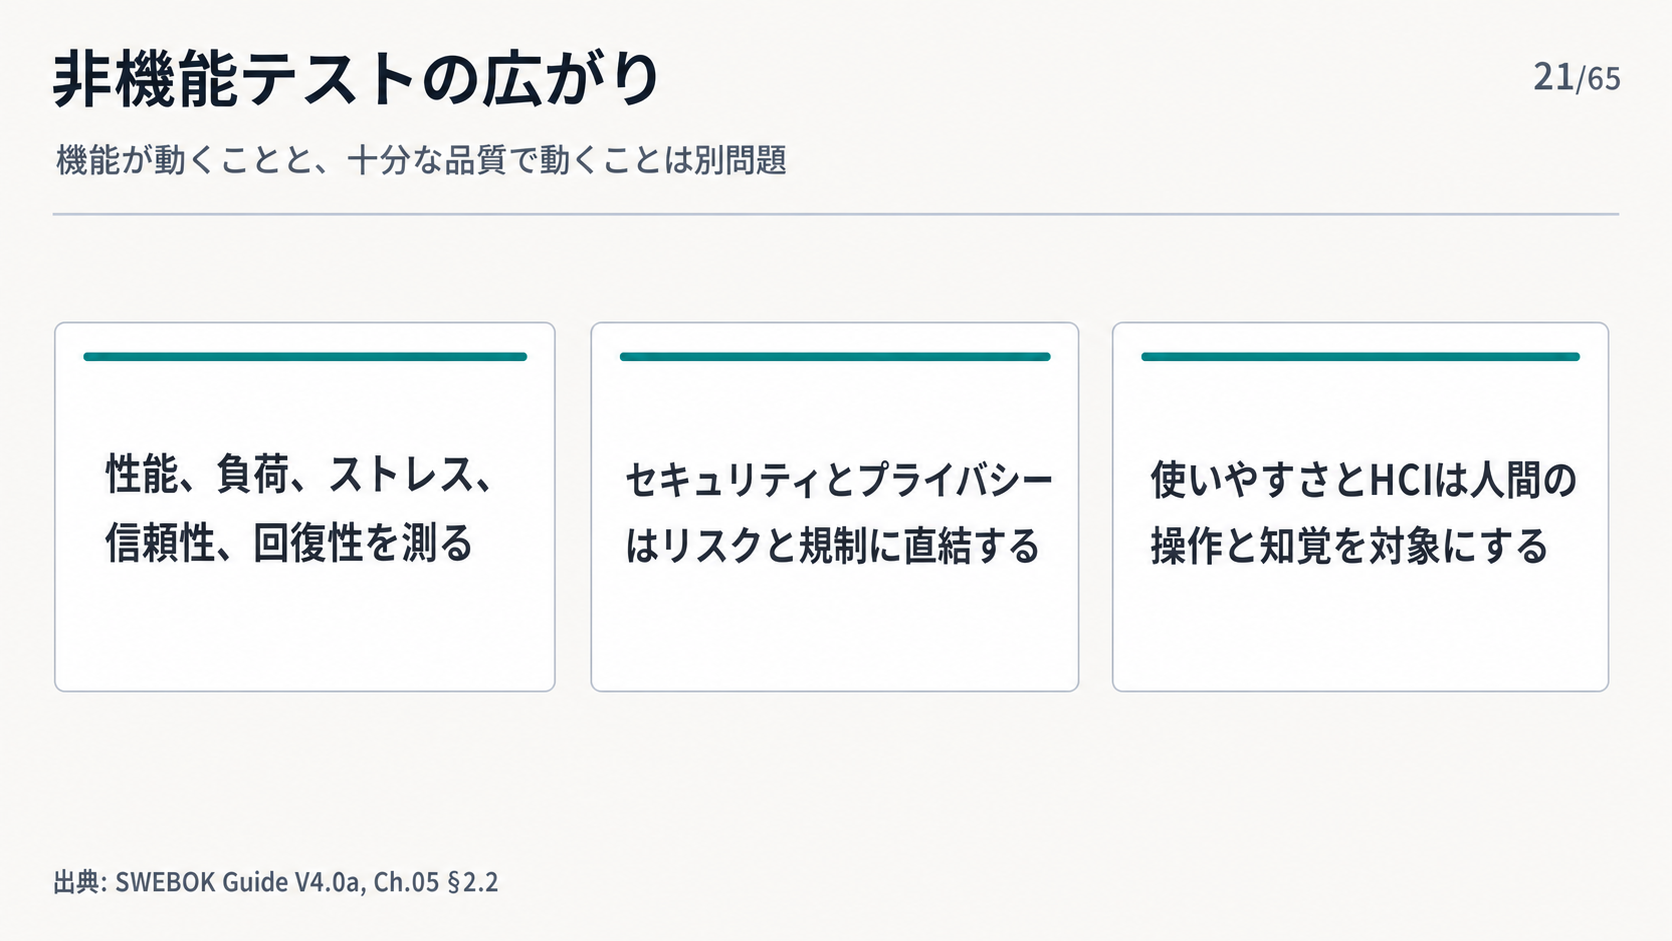
\includegraphics[width=0.96\linewidth]{assets/fig-ch05-01.png}}{\fbox{\parbox[c][48mm][c]{0.9\linewidth}{\centering 画像生成待ち\\05 章の全体地図}}}
\caption{05 章の全体地図}
\label{fig:ch05-01}
\end{figure}

% Source: tex/chapters/ch05/02_最初に必要な用語.tex
\subsection*{最初に必要な用語}
\addcontentsline{toc}{subsection}{最初に必要な用語}
\par\smallskip\noindent\refstepcounter{table}\label{tab:ch05-01}\textbf{表 \thetable: 第05章 ソフトウェアテスト 表01}\par\smallskip
\begin{longtable}{P{0.23\linewidth}P{0.69\linewidth}}
\toprule
\textbf{用語} & \textbf{初学者向けの説明} \\
\midrule
テスト対象システム SUT & テストされる対象である。プログラム、アプリケーション、サービス、マイクロサービス、ミドルウェア、システム、システム群、エコシステムまで含み得る。\\
テストケース & 入力値だけでなく、実行条件、時刻条件、手順、期待結果を含む、テスト実行のための具体的な指定である。\\
テストスイート & 複数のテストケースをまとめた集合である。\\
期待結果 & テストを実行したときに、本来得られるべき出力、状態変化、メッセージ、振る舞いである。\\
テストオラクル & 実際の結果が正しいかどうかを判定する基準または仕組みである。人、仕様、モデル、コード注釈、比較ツールなどがなり得る。\\
欠陥 & 障害を引き起こす原因である。コード、設計、要求、設定、運用手順に存在し得る。\\
障害 & 利用者や外部から観測される望ましくない振る舞いである。欠陥が存在しても、条件がそろわなければ障害として現れないことがある。\\
カバレッジ & テストが対象のどの部分をどれだけ通ったかを表す度合いである。文、分岐、条件、要求、状態など、対象は目的によって変わる。\\
回帰テスト & 変更後に、以前できていたことが壊れていないかを再確認するテストである。\\
シフトレフト & テストや品質確認を開発の後半に置くだけでなく、早い段階から行う考え方である。\\
\bottomrule
\end{longtable}

% Source: tex/chapters/ch05/03_導入：ソフトウェアテストとは何か.tex
\subsection*{導入：ソフトウェアテストとは何か}
\addcontentsline{toc}{subsection}{導入：ソフトウェアテストとは何か}
ソフトウェアテストとは、通常は無限に近い実行領域から有限個のテストケースを選び、テスト対象システムが期待される振る舞いを提供するかを動的に確認する活動である。この定義には、いくつかの重要な意味が含まれる。

第一に、テストは動的である。つまり、対象を実行して確認する。静的解析、レビュー、形式的証明などは品質向上に重要であるが、この章では主に実行を伴うテストを扱う。

第二に、テストは有限である。すべての入力値、すべての状態、すべての環境を試すことは現実的でない。したがって、テストでは、限られた時間、費用、人員の中で、どのテストケースを選ぶかを決める必要がある。

第三に、テストには期待結果が必要である。実行結果を見ても、それが正しいかどうかを判断できなければテストにならない。期待結果を判断する仕組みがテストオラクルである。

\begin{figure}[htbp]
\centering
\IfFileExists{assets/fig-ch05-02.png}{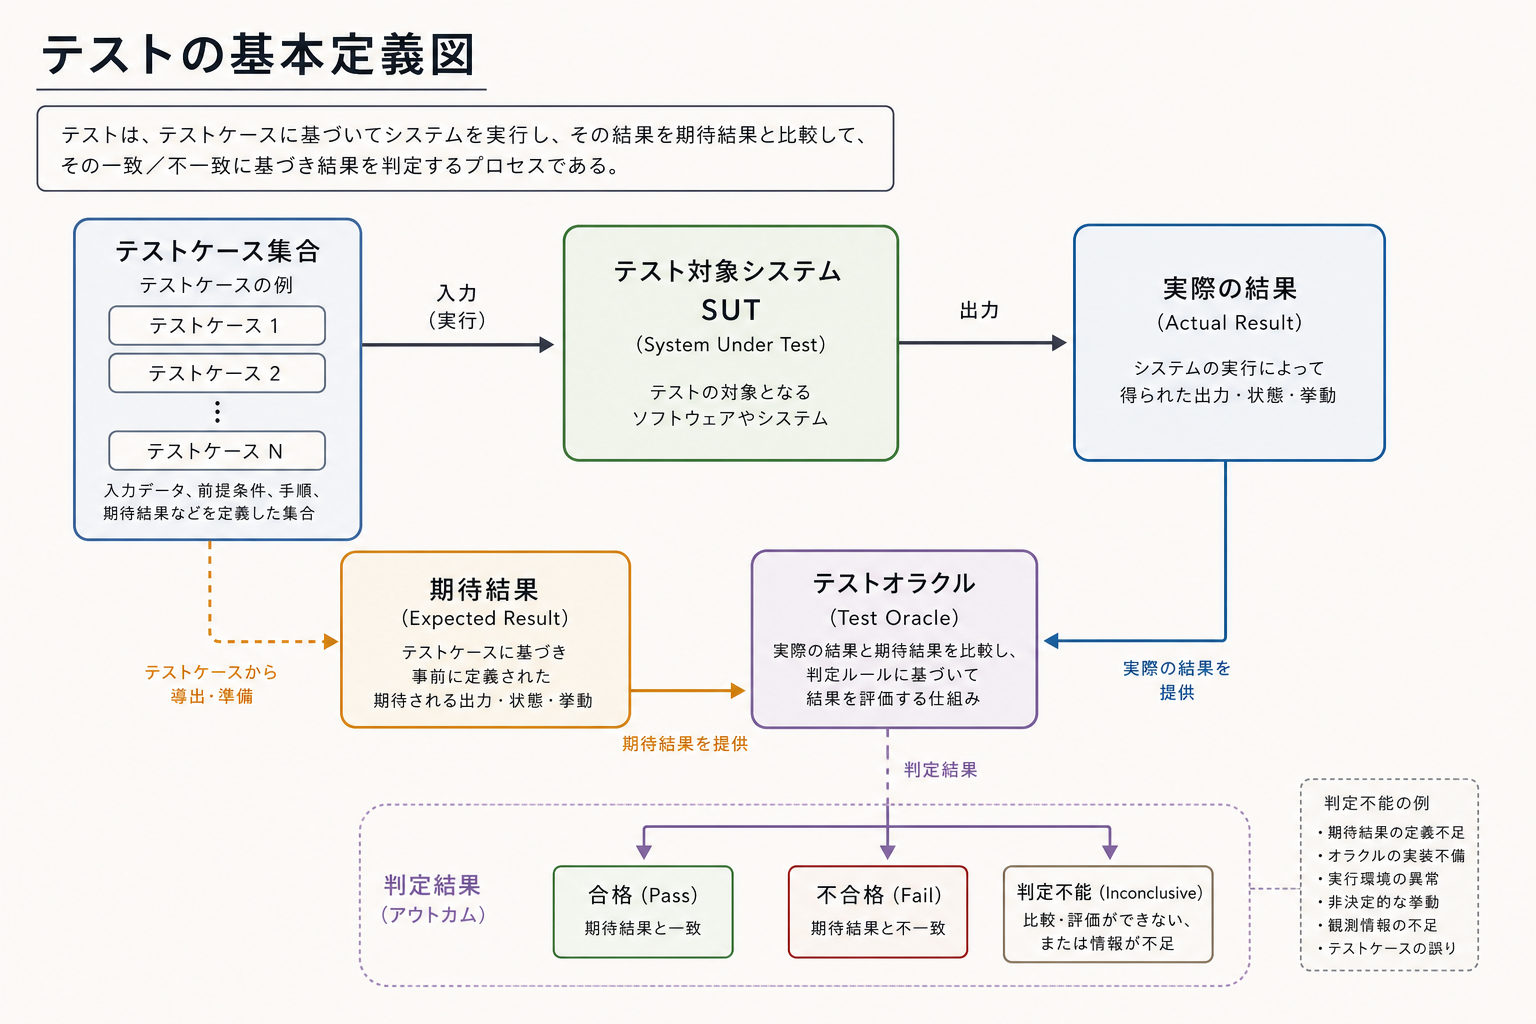
\includegraphics[width=0.96\linewidth]{assets/fig-ch05-02.png}}{\fbox{\parbox[c][48mm][c]{0.9\linewidth}{\centering 画像生成待ち\\テストの基本定義図}}}
\caption{テストの基本定義図}
\label{fig:ch05-02}
\end{figure}
